\subsection{Modelos de crecimiento con tasas de ahorro exógeno (el modelo Solow-Swan}

\subsubsection{La estructura básica}

En el mundo real, la producción se lleva a cabo utilizando muchos insumos diferentes para la producción. Resumimos todos ellos en solo tres: capital físico $K\left(t\right)$, trabajo $L\left(t\right)$ y conocimiento $T\left(t\right)$. La función de producción tiene la forma:
\begin{equation}
Y\left(t\right)=F\left[K\left(t\right), L\left(t\right), T\left(t\right)\right]
\end{equation}
donde $Y(t)$ es el flujo de salida producido en el tiempo $t$.

El capital, $K\left(t\right)$, representa las entradas físicas duraderas, como máquinas, edificios, lápices, y así.

La segunda entrada a la función de producción es mano de obra, $L\left(t\right)$, y representa las entradas asociado con el cuerpo humano. Esta entrada incluye la cantidad de trabajadores y la cantidad de tiempo que trabajan, así como su fuerza física, habilidades y salud.

La tercera entrada es el nivel de conocimiento o tecnología, $T\left(t\right)$. Trabajadores y máquinas no puede producir nada sin una fórmula o modelo que les muestre cómo hacerlo.

Asumimos un sector de la tecnología de producción en la que lasalida es un bien homogéneo que puede consumirse, $C\left(t\right)$ o invertirse, $I\left(t\right)$. La inversión se utiliza para crear nuevas unidades de capital físico, $K\left(t\right)$, o para reemplazar el capital viejo.

En una economía cerrada sin gasto público, toda la producción se dedica al consumo o la inversión bruta, $Y\left(t\right)=C\left(t\right)+I\left(t\right)$. Al restar $C\left(t\right)$ de ambos lados y darse cuenta de que la producción es igual a ingresos, obtenemos que, en esta economía simple, la cantidad ahorrada, $S\left(t\right)\equiv Y\left(t\right)-C\left(t\right)$, es igual a la cantidad invertida, $I\left(t\right)$.

Sea $s\left(\cdot\right)$ la fracción de salida que se guarda, es decir, la \emph{tasa de ahorro}, de modo que $1-s\left(\cdot\right)$ es la fracción de salida que es consumida. 

Supongamos que $s\left(\cdot\right)$ se da de forma exógena. La función más simple, la asumida por Solow (1956) y Swan (1956) en sus clásicos artículos, es una constante, $0\leq s\left(\cdot\right)=s\leq1$.

Dado que el ahorro debe ser igual a la inversión, $S\left(t\right)=I\left(t\right)$, se sigue que la \emph{tasa de ahorro} es igual a la \emph{tasa de inversión}. En otras palabras, la tasa de ahorro de una economía cerrada representa la fracción del PBI que otra economía dedica a la inversión.

Supongamos que el capital es un bien homogéneo que se deprecia a una tasa constante $\delta>0$, es decir, en cada momento, una fracción constante del stock de capital se desgasta y, por lo tanto, ya no se puede usar para la producción. Sin embargo, antes de evaporarse, todas las unidades de capital son asumidas igualmente productivas, independientemente de cuándo se produjeron originalmente.

\begin{remark}
En una economía abierta con gastos gubernamentales, la condición es \[ Y\left(t\right)-r\cdot D\left(t\right)=C\left(t\right)+I\left(t\right)+G\left(t\right)+N X\left(t\right) \] donde $D\left(t\right)$ es la deuda internacional, $r$ es la tasa de interés internacional real, $G\left(t\right)$ es el gasto público y $N X\left(t\right)$ son las exportaciones netas. Asumiremos que no existe gasto público, así que $G\left(t\right)=0$, y la economía es cerrada, así que $D\left(t\right)=N X\left(t\right)=0$.
\end{remark}

El incremento neto en el stock de capital físico en un momento es igual a la inversión bruta menos depreciación:
\begin{equation}
\dot{K}\left(t\right)=I\left(t\right)-\delta K\left(t\right)=s\cdot F\left[K\left(t\right),L\left(t\right),T\left(t\right)\right]-\delta K\left(t\right)
\end{equation}
donde el punto sobre una variable, como $\dot{K}\left(t\right)$, denota la diferenciación con respecto al tiempo, $\dot{K}\left(t\right)\equiv\partial K\left(t\right)/\partial t$ y $0\leq s\leq1$. La ecuación (1.2) determina la dinámica de $K$ para una determinada tecnología y mano de obra.

El entrada trabajo, $L$, varía con el tiempo debido al crecimiento de la población, los cambios en la tasa de participación, cambios en la cantidad de tiempo trabajado por el trabajador típico y mejoras en las habilidades y calidad de los trabajadores. Nosotros simplificamos asumiendo que todos trabajan la misma cantidad de tiempo y que todos tienen la misma habilidad constante, el cual normalizamos a uno. Por lo tanto, identificamos el aporte laboral con la población total.

El crecimiento de la población refleja el comportamiento de la fertilidad, la mortalidad y la migración, pero simplificamos suponiendo que la población crece a una tasa constante, tasa exógena, $\dot{L}/L=n\geq0$, sin utilizar ningún recurso. Si nos normalizamos el número de personas en el tiempo $0$ a $1$ y la intensidad del trabajo por persona también a $1$, luego la población y fuerza laboral en el momento $t$ son iguales a
\begin{equation}
L\left(t\right)=e^{nt}.
\end{equation}
Para resaltar el papel de la acumulación de capital, comenzamos con el supuesto de que el nivel de tecnología, $T\left(t\right)$, es una constante. Esta suposición se relajará más tarde.

Si $L\left(t\right)$ proviene de la ecuación (1.3) y el progreso tecnológico está ausente, entonces la ecuación (1.2) determina las rutas de tiempo de capital, $K\left(t\right)$ y la salida, $Y\left(t\right)$. Una vez que sepamos cómo el capital o el PIB cambian con el tiempo, también se determinan las tasas de crecimiento de estas variables. En las siguientes secciones, mostramos que este comportamiento depende de manera crucial de las propiedades de función de producción, $F\left(\cdot\right)$.

\subsection{El neoclásico modelo de Solow y Swan}

\subsubsection{La neoclásica función de producción}

El proceso del crecimiento económico depende de la forma de la función de producción. Nosotros inicialmente consideramos la función de producción neoclásica. Decimos que una función de producción, $F\left(K,L,T\right)$, es \emph{neoclásica} si se cumplen las siguientes propiedades:
\begin{description}
	\item[Rendimientos de escala constantes.] La función $F\left(\cdot\right)$ exhibe rendimientos de escala constantes. Es decir, si multiplicamos el capital y el trabajo por la misma constante positiva, $\lambda$, obtenemos $\lambda$ veces la cantidad de salida:
	\begin{equation}
	F\left(\lambda K,\lambda L,T\right)=\lambda\cdot F\left(K,L,T\right)\quad\text{para todo }\lambda>0.
	\end{equation}
	Esta propiedad también se conoce como \emph{homogeneidad de grado uno en} $K$ \emph{y} $L$. Es importante tener en cuenta que la definición de escala incluye solo los dos insumos rivales: capital y trabajo. En otras palabras, no definimos rendimientos de escala constantes como $F\left(\lambda K,\lambda L,\lambda T\right)=\lambda\cdot F\left(K,L,T\right)$.
	\item[Retornos positivos y decrecientes a los insumos privados.] Para todos $K>0$ y $L>0$, $F\left(\cdot\right)$ exhibe productos marginales positivos y decrecientes con respecto a cada entrada:
	\begin{equation}
	\begin{split}
	\frac{\partial F}{\partial K}>0,\quad&\frac{\partial^{2}F}{\partial K^{2}}<0\\
	\frac{\partial F}{\partial L}>0,\quad&\frac{\partial^{2}F}{\partial L^{2}}<0
	\end{split}
	\end{equation}
Así, la tecnología neoclásica supone que, manteniendo constantes los niveles de tecnología y trabajo, cada unidad adicional de capital ofrece adiciones positivas a la producción, pero estas adiciones disminuyen a medida que aumenta el número de máquinas. Se asume la misma propiedad para el trabajo.
\item[Condiciones de Inada.] La tercera característica definitoria de la función de producción neoclásica es que el producto marginal del capital (o trabajo) se acerca al infinito como capital (o trabajo) va a $0$ y se acerca a $0$ cuando el capital (o trabajo) va al infinito:
\begin{equation}
\begin{split}
\lim\limits_{K\to0}\left(\frac{\partial F}{\partial K}\right)=\lim\limits_{L\to0}\left(\frac{\partial F}{\partial L}\right)=\infty,
\lim\limits_{K\to\infty}\left(\frac{\partial F}{\partial K}\right)=\lim\limits_{L\to\infty}\left(\frac{\partial F}{\partial L}\right)=\infty.
\end{split}
\end{equation}
Estas últimas propiedades son llamadas \emph{condiciones de Inada}, siguiendo a Inada (1963).
\item[Esencialidad.] Algunos economistas agregan el supuesto de \emph{esencialidad} a la definición de una función de producción neoclásica. Una entrada es esencial si se necesita estrictamente una cantidad positiva para producir una cantidad positiva de salida. Mostramos en el apéndice que las tres propiedades neoclásicas en las ecuaciones (1.4)-(1.6) implican que cada entrada es esencial para la producción, es decir, $F\left(0,L\right)=F\left(K,0\right)=0$. Las tres propiedades de la función de producción neoclásica también implican que la salida va al infinito cuando cualquier entrada va al infinito, otra propiedad que es probada en el apéndice.
\end{description}

\begin{description}
	\item[Variables per cápita] Cuando decimos que un país es rico o pobre, tendemos a pensar en condiciones de producción o consumo por persona. En otras palabras, no creemos que India sea más rico que los Países Bajos, a pesar de que India produce mucho más PBI, porque, una vez que dividido por el número de ciudadanos, la cantidad de ingresos que cada persona obtiene en promedio es mucho más pequeño en la India que en los Países Bajos. Para capturar esta propiedad, construimos el modelo en términos per cápita y estudiamos principalmente el comportamiento dinámico de las cantidades per cápita del PBI, consumo y capital.
\end{description}

Dado que la definición de rendimientos de escala constantes se aplica a todos los valores de $\lambda$, también se aplica a $\lambda=1/L$. Por lo tanto, la salida se puede escribir como
\begin{equation}
Y=F\left(K,L,T\right)=L\cdot F\left(K/L,1,T\right)=L\cdot f\left(k\right)
\end{equation}
donde $k\equiv K/L$ es el capital por trabajador, $y\equiv Y/L$ es la salida por trabajador, y la función $f\left(k\right)$ es definido para ser igual a $F\left(k,1,T\right)$. Este resultado significa que la función de producción puede expresarse en \emph{forma intensiva} (esto es, en forma \emph{por trabajador} o \emph{per cápita}) como
\begin{equation}
y=f\left(k\right)
\end{equation}
En otras palabras, la función de producción no exhibe ``efectos de escala'': la producción por persona es determinado por la cantidad de capital físico al que cada persona tiene acceso, manteniéndose constante $k$, teniendo más o menos o menos trabajadores no afecta la producción total por persona.

Podemos diferenciar esta condición $Y=L\cdot f\left(k\right)$ con respecto a $K$, para $L$ fijo, y luego con respecto a $L$, para $K$ fijo, para verificar que los productos marginales de los factores de entrada son dados por
\begin{align}
\frac{\partial Y}{\partial K}&=f^{\prime}\left(k\right).\\
\frac{\partial Y}{\partial L}&=f\left(k\right)-k\cdot f^{\prime}\left(k\right).
\end{align}
%\begin{figure}
%	\centering
%	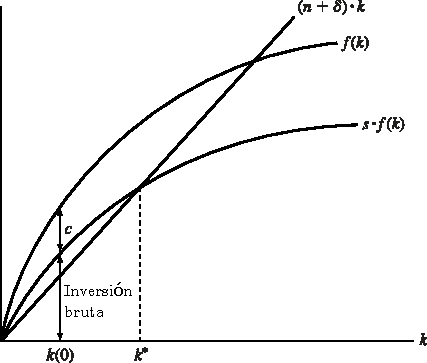
\includegraphics{figs/investment.pdf}
%	\caption{\textbf{El modelo de Solow-Swan.} La curva de la inversión bruta, $s\cdot f\left(k\right)$ es proporcional a la función de producción, $f\left(k\right)$. El consumo por persona es igual a la distancia vertical entre $f\left(k\right)$ y $s\cdot f\left(k\right)$. La depreciación efectiva (para $k$) es dada por $\left(n+\delta\right)\cdot k$, una línea recta desde el origen. El cambio en $k$ es dado por la distancia vertical entre $s\cdot f\left(k\right)$ y $\left(n+\delta\right)\cdot k$. El nivel de estado estacionario del capital, $k^{\ast}$, está determinado en la intersección de la curva $s\cdot f\left(k\right)$ con la recta $\left(n+\delta\right)\cdot k$.}
%\end{figure}

Las condiciones de Inada implican que $\lim\limits_{k\to0}\left[f^{\prime}\left(k\right)\right]=\infty$ y $\lim\limits_{k\to\infty}\left[f^{\prime}\left(k\right)\right]=0$. La figura 1.1 muestra la producción neoclásica en términos per cápita: pasa por el origen; es vertical en cero, pendiente hacia arriba y cóncavo; y su pendiente es asíntota a cero cuando $k$ va al infinito.
\begin{description}
\item[Un ejemplo de Cobb-Douglas] Una función de producción simple que a menudo se piensa que proporciona una descripción razonable de las economías reales es la función Cobb-Douglas,
\end{description}
\begin{equation}
Y=AK^{\alpha}L^{\left(1-\alpha\right)}
\end{equation}
donde $A>0$ es el nivel de la tecnología y $\alpha$ es una constante con $0<\alpha<1$. La función Cobb-Douglas se puede escribir en forma intensiva como
\begin{equation}
y=Ak^{\alpha}
\end{equation}
Note que $f^{\prime}\left(k\right)=A\alpha k^{\alpha-1}>0$, $f^{\prime\prime}\left(k\right)=-A\alpha\left(1-\alpha\right)k^{\alpha-2}<0$, $\lim\limits_{k\to\infty}f^{\prime}\left(k\right)=0$ y $\lim\limits_{k\to0}f^{\prime}=\infty$. Por lo tanto, la forma Cobb-Douglas satisface las propiedades de una función neoclásica de producción.

La propiedad clave de la función de producción de Cobb-Douglas es el comportamiento del factor de participación en los ingresos. En una economía competitiva, el capital y el trabajo, cada uno recibe sus productos marginales, esto es, el producto marginal del capital es igual al precio de alquiler $R$, y el producto marginal del trabajo es igual a la tasa salarial $w$. Por lo tanto, cada unidad de capital se paga $R=f^{\prime}\left(k\right)=\alpha Ak^{\alpha-1}$, y cada unidad de trabajo se paga $w=f\left(k\right)-k\cdot f^{\prime}\left(k\right)=\left(1-\alpha\right)\cdot Ak^{\alpha}$. El capital compartido de ingreso es entonces $Rk/f\left(k\right)=\alpha$, y el trabajo compartido es $w/f\left(k\right)=1-a$. Por lo tanto, en un entorno competitivo, los factor de ingresos compartidos son constantes, independiente de $k$--cuando la función de producción es Cobb-Douglas.

\subsubsection{La ecuación fundamental del modelo de Solow-Swan}

Ahora analizamos el compartamiento dinámico de la economía descrita por la función de producción neoclásica. El modelo del crecimiento resultante es llamado el modelo de Solow--Swan, después de las importantes contribuciones de Solow (1956) y Swan (1956).

El cambio en el capital principal sobre el tiempo está dado por la ecuación (1.2). Si dividimos ambos lados de esta ecuación por $L$, obtenemos \[ \dot{K}/L=s\cdot f\left(k\right)-\delta k. \] El lado derecho de la ecuación contiene solo variables per cápita, pero el lado izquierdo no. Así, este no es una ecuación diferencial ordinaria que pueda ser fácilmente resuelta. Con el fin de transforma esta en una ecuación diferencial en términos de $k$, podemos tomar la derivada $k\equiv K/L$ con respecto al tiempo para obtener \[ \dot{k}=\frac{d\left(K/L\right)}{dt}=\frac{\dot{K}}{L}-nk \] donde $n=\frac{\dot{L}}{L}$. Si sustituimos este resultado en la expresión para $\frac{\dot{K}}{L}$, podemos reagrupar para obtener
\begin{equation}
\dot{k}=s\cdot f\left(k\right)-\left(n+\delta\right)\cdot k
\end{equation}
La ecuación (1.13) es la ecuación diferencial fundamental del modelo de Solow--Swan. Esta ecuación no lineal depende solo de $k$.

El término $n+\delta$ en el lado derecho de la ecuación (1.13) puede ser pensado como la tasa de depreciación efectiva para el cociente capital--trabajo, $k\equiv K/L$. Si la tasa de ahorro, $s$, fuera $0$, el capital por persona disminuiría en parte debido a la depreciación del capital a la tasa $\delta$ y parcialmente debido al incremento en el número de persona a la tasa $n$.

La figura 1.1 muestra el funcionamiento de la ecuación (1.13). La curva superior es la función de producción, $f\left(k\right)$. El término $\left(n+\delta\right)\cdot k$, que aparece en la ecuación (1.13), es dibujado en la figura 1.1 como una línea recta desde el origen con pendiente positiva $n+\delta$. Los términos $s\cdot f\left(k\right)$ en la ecuación (1.13) se parece a la función de producción excepto por la multiplicación de una fracción positiva $s$. Note de la figura que la curva $s\cdot f\left(k\right)$ empieza en el origen [porque $f\left(0\right)=0$], tiene pendiente positiva [porque $f^{\prime}\left(k\right)>0$], y se hace más horizontal cuando $k$ aumenta [porque $f^{\prime\prime}\left(k\right)<0$]. Las condiciones de Inada implican que la curva $s\cdot f\left(k\right)$ es vertical en $k=0$ y se volverá horizontal cuando $k$ va al infinito. Estas propiedades implican que, aparte del origen, la curva $s\cdot f\left(k\right)$ y la recta $\left(n+\delta\right)\cdot k$ cruza una y solo una vez.

Considere una economía con el capital social por persona $k\left(0\right)>0$. La figura 1.1 muestra la inversión bruta persona es igual a la altura de la curva $s\cdot f\left(k\right)$ en este punto. El consumo por persona iguala la diferencia vertical en este punto entre las curvas $f\left(k\right)$ y $s\cdot f\left(k\right)$.
